% $Header$
% $Author: fager $
% $Date: 2004-10-21 20:59:19 +0200 (Thu, 21 Oct 2004) $
% $Revision: 223 $
% $Log$
% Revision 1.2  2004/10/21 18:59:06  fager
% Version logging added. Comments from KA implemented.
%

\section{Plotting functions}
Finally, some useful functions for plotting \verb"meassp" and
\verb"meassweep" data are described.

\subsection{Combined Smith/polar diagram}
A combined Smith/polar diagram for depicting two-port S-parameters
is easily produced with the \verb"smithplot" function. It takes a
\verb"meassp" object as input and generates a combined Smith/polar
plot for all four S-parameters (See \figref{Smith}):
\begin{small}
\begin{verbatim}
    >> smithplot(msp);
\end{verbatim}
\end{small}

\begin{figure}[htbf]
    \centering
  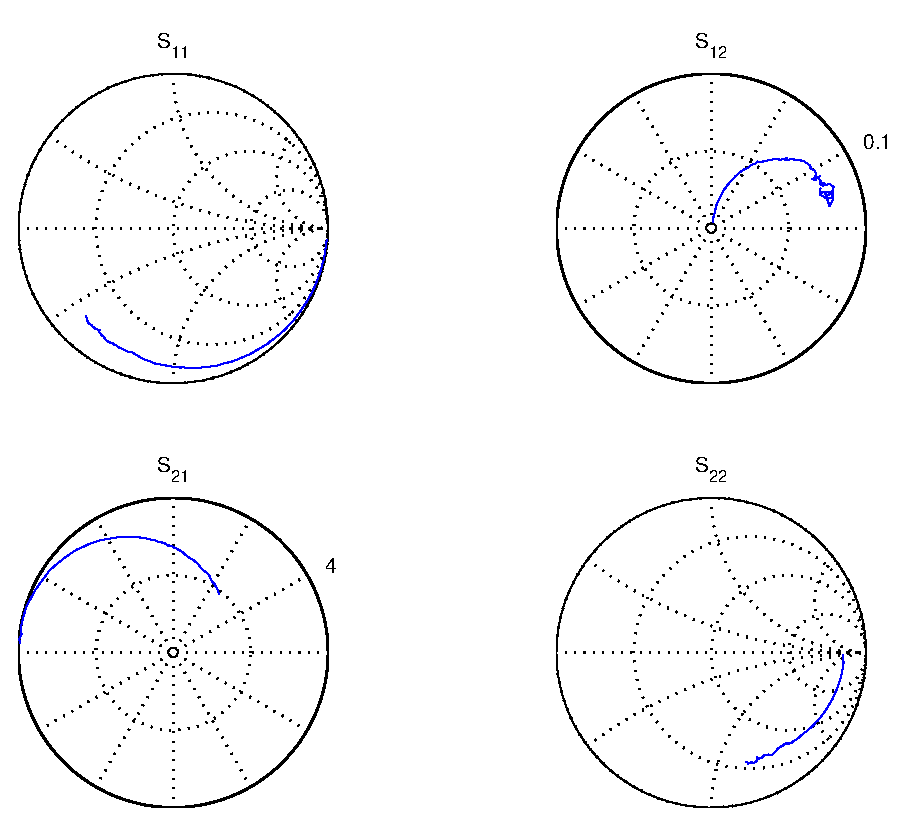
\includegraphics[scale=0.6]{Figures/Smith.eps}
  \caption{Combined Smith/polar diagram produced with smithplot.}\label{fig:Smith}
\end{figure}

\subsection{Single parameter plot}
Single parameters may be plotted using the \verb"paramplot"
command. It is particularly useful for producing single parameter
Smith plots. The syntax for this is given below.
\begin{small}
\begin{verbatim}
    >> paramplot(msp,'S11','smith',gca);
\end{verbatim}
\end{small}
Other plotting methods are available as described in the help at
\newline \verb">> help paramplot".

\subsection{Swept data}
A modified \verb"plot" function has been implemented to plot
parameters of \verb"meassweep" object against each other. This is
useful for producing I/V plots from the biasing information
contained in the measurement files. The syntax is exemplified by,
\begin{small}
\begin{verbatim}
    >> plot(sweep,'Vgs','Ids')
\end{verbatim}
\end{small}
The plot produced is shown in \figref{IdsVgs}.

\begin{figure}[htbf]
    \centering
  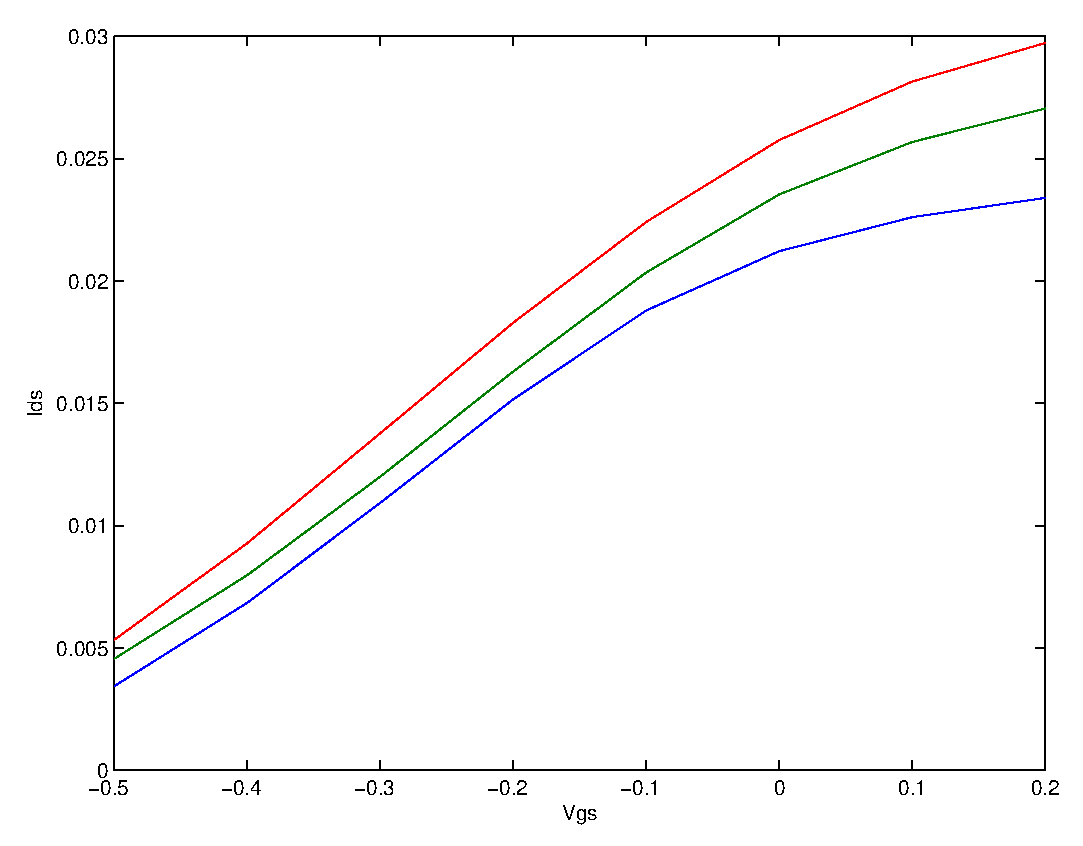
\includegraphics[scale=0.6]{Figures/IdsVgs.eps}
  \caption{Ids-Vgs characteristics produced with the meassweep-plot function.}\label{fig:IdsVgs}
\end{figure}
